\begin{figure}
    \begin{center}
    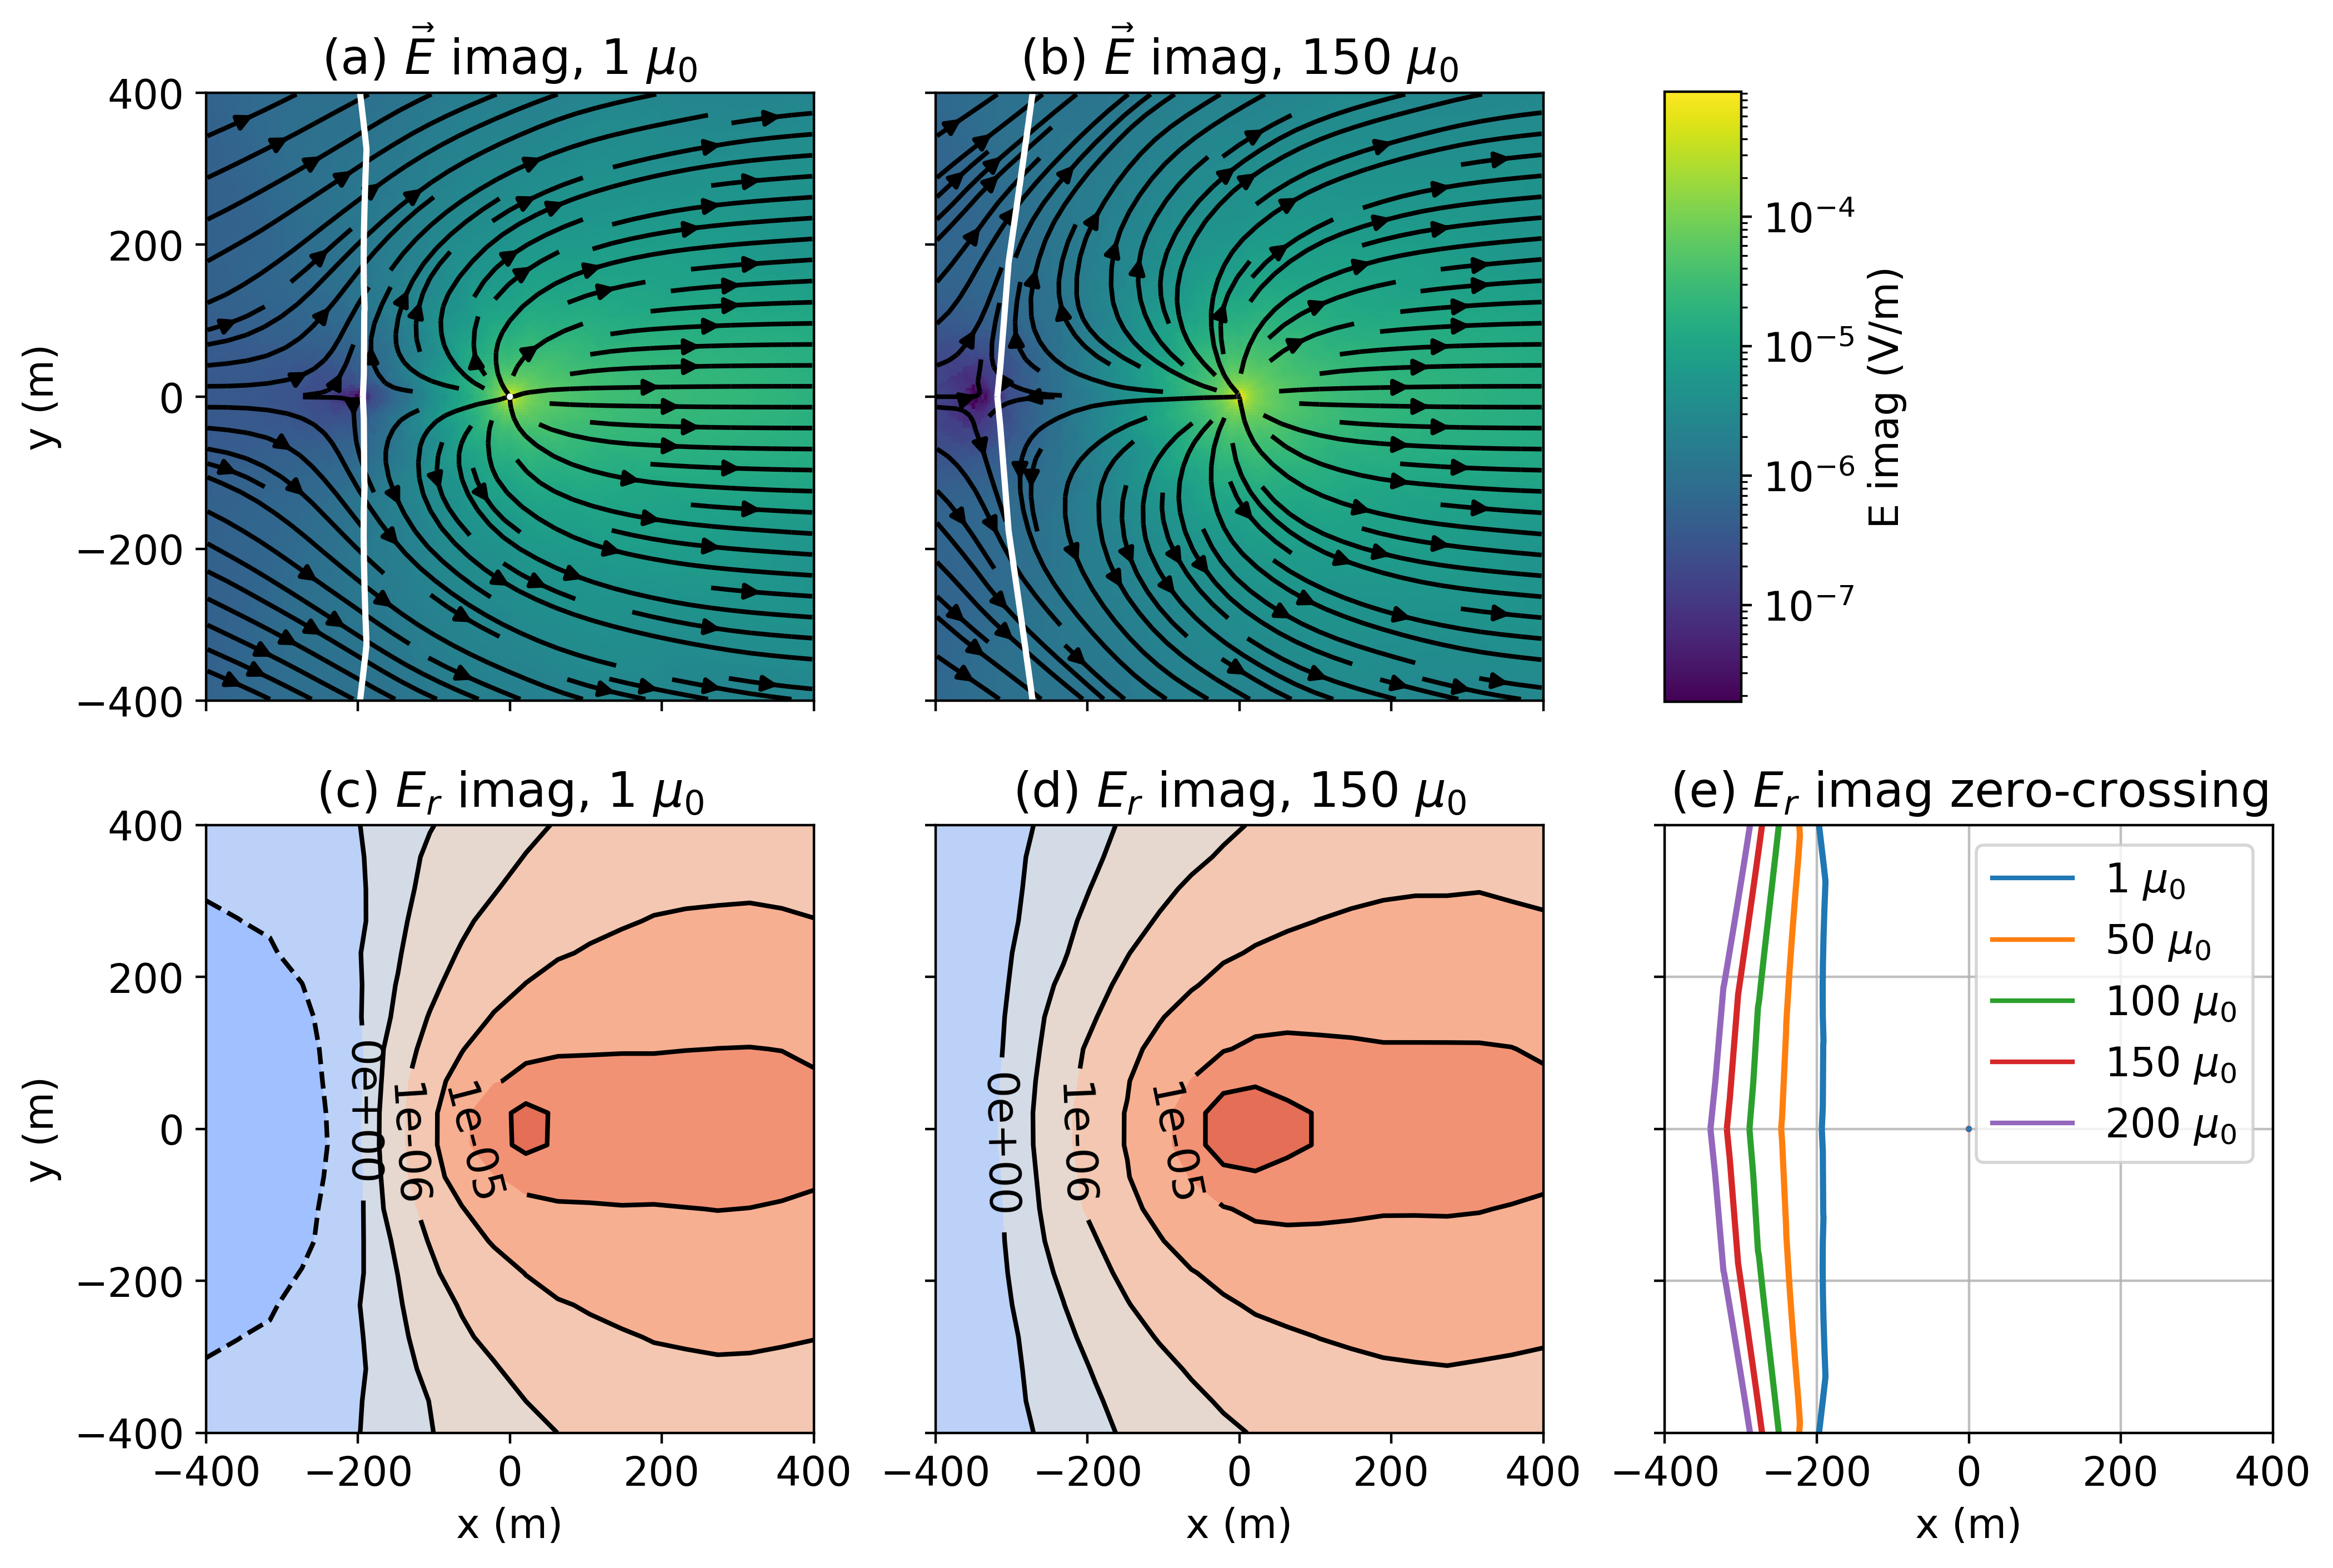
\includegraphics[width=\textwidth]{figures/zero-crossing-permeability.png}
    \end{center}
\caption{
    Depth slice of the imaginary component of the electric field just beneath the surface (z=-2.5m) for (a) a well with $\mu_r=1$ and (b) a well with $\mu_r=150$. The white line denotes the contour where the radial electric field is zero. In (c) and (d) we show contours of the radial electric field; red denotes positive values and blue are negative. In (e), we show the location of the zero-crossing for a range of casing permeabilities. The well is located at the origin (x=0m, y=0m). The transmitter wire runs from x=0m to x=500m along the y=0 line, as was shown in Figure \ref{fig:setup}a.
}
\label{fig:zero-crossing-permeability}
\end{figure}



